\documentclass[conference]{IEEEtran}
\IEEEoverridecommandlockouts

\usepackage{cite}
\usepackage{amsmath,amssymb}
\usepackage{booktabs}
\usepackage{graphicx}
\usepackage{xcolor}
\usepackage{url}
\usepackage{balance}

\graphicspath{{figures/}}
\newcommand{\method}{\textsc{Value-CQAG}}
\newcommand{\memit}{\textsc{MEMIT}}

\title{Locality-Aware Activation Intervention for Multi-Hop Factual Adaptation in Large Language Models}

% Replace the anonymous author block with the camera-ready author metadata.
\author{\IEEEauthorblockN{Anonymous Authors}}

\begin{document}
\maketitle

\begin{abstract}
Large language models can be adapted to counterfactual facts without changing their parameters, but multi-hop factual updates often trade answer quality for unintended changes on unrelated inputs. We study this trade-off through \method{}, a content-routed activation intervention that acts as an auditable signal path: it injects edited values only when a question overlaps the edited context. Across a frozen 100-case, 300-question MQuAKE-CF confirmation pool, \method{} improves question-level generation from 2.00\% to 38.67\% on Qwen2.5-7B and from 4.00\% to 51.33\% on Llama-3.1-8B, while its end-to-end exact-output locality on a 10,000-pair audit is 98.49\%. We compare against explicit facts, retrieval-plus-in-context learning, and parameter editing with \memit{}. The Qwen retrieval control reaches 95.0\% question-level generation but substantially lower exact locality, whereas \memit{} reaches only 16.0\% and 14.33\% on the two models. Error audits separate router misses from residual old answers and multi-hop entity errors. The results position activation intervention as a controllable signal path for factual adaptation, rather than as a replacement for retrieval or a new state-of-the-art knowledge editor.
\end{abstract}

\begin{IEEEkeywords}
large language models, factual adaptation, activation intervention, locality, multi-hop reasoning, generative AI
\end{IEEEkeywords}

\section{Introduction}
Large language models (LLMs) store factual associations in distributed internal representations and can answer multi-hop questions by composing those associations. Updating one fact, however, can expose a difficult systems trade-off: the intervention must affect questions that depend on the edited fact while leaving unrelated generations unchanged. This is especially important for applications that require rapid, reversible adaptation without modifying model weights.

Existing knowledge-editing methods modify parameters directly, for example by locating and rewriting factual associations in feed-forward layers \cite{geva2021transformer,meng2022rome,meng2023memit}. Retrieval and in-context methods avoid parameter changes but can introduce long prompts and broad interference \cite{lewis2020rag,zheng2023ike}. These comparisons are often made using a single success number, which obscures whether a failure comes from missing the relevant context, retaining the old answer, or choosing an incorrect entity during multi-hop composition.

We present a controlled study of \method{}, a value-level activation intervention with a content-token router. The router computes overlap between the current question and the edited context; only questions above a fixed threshold receive the intervention. The method is deliberately conservative: the model remains frozen, the intervention is prompt-only, and locality is measured on a separate question set. Figure~\ref{fig:pipeline} summarizes the evaluation path.
This separation of routing, intervention, and generation makes the method amenable to signal-path analysis: false routes can be measured independently from downstream multi-hop reasoning failures.

Our contributions are:
\begin{itemize}
    \item A locality-aware activation intervention for multi-hop factual adaptation that separates routing from generation and does not update model weights.
    \item A controlled cross-model evaluation on Qwen2.5-7B and Llama-3.1-8B with the same frozen confirmation pool, explicit-fact and retrieval controls, and \memit{} baselines.
    \item A 10,000-pair end-to-end locality audit and a failure decomposition that distinguishes router misses, old-answer residuals, and entity/reasoning errors.
\end{itemize}

\section{Method}
\subsection{Problem setup}
Let $\mathcal{E}=\{(s_i,r_i,o_i^{\mathrm{new}})\}$ be a set of edited subject--relation--object facts and let $q$ be a question whose answer may require several facts. The base model $f_\theta$ is frozen. We seek a conditional intervention $\Delta(q,\mathcal{E})$ such that
\begin{equation}
    \hat{y}=f_\theta(q;\Delta(q,\mathcal{E}))
\end{equation}
is consistent with the edited facts, while $f_\theta(q;0)$ is retained for unrelated questions. This differs from parameter editing, which produces a single edited model $f_{\theta+\Delta\theta}$ for all subsequent inputs.

\subsection{Content-token routing}
We represent the edit context and the question as sets of normalized content tokens, removing stop words and punctuation. The router score is the Jaccard overlap
\begin{equation}
    \rho(q,\mathcal{E}) = \frac{|T(q)\cap T(\mathcal{E})|}{|T(q)\cup T(\mathcal{E})|}.
\end{equation}
An intervention is enabled when $\rho\geq\tau$, with $\tau=0.35$ fixed on development data. The threshold is not tuned on the confirmation pool. A routed miss is counted separately from a generation error after a route.

\subsection{Prompt-only value intervention}
When routed, the intervention supplies the edited values as a compact prompt-side context at the model input. It is applied during the prompt encoding pass and is not repeatedly injected into later autoregressive decoding steps. This design choice is empirical: continuing the intervention for the first two generated tokens decreases question-level generation by 4.00 percentage points on Qwen and 7.00 points on Llama. Prompt-only intervention therefore provides the primary method reported here.

\begin{figure}[t]
    \centering
    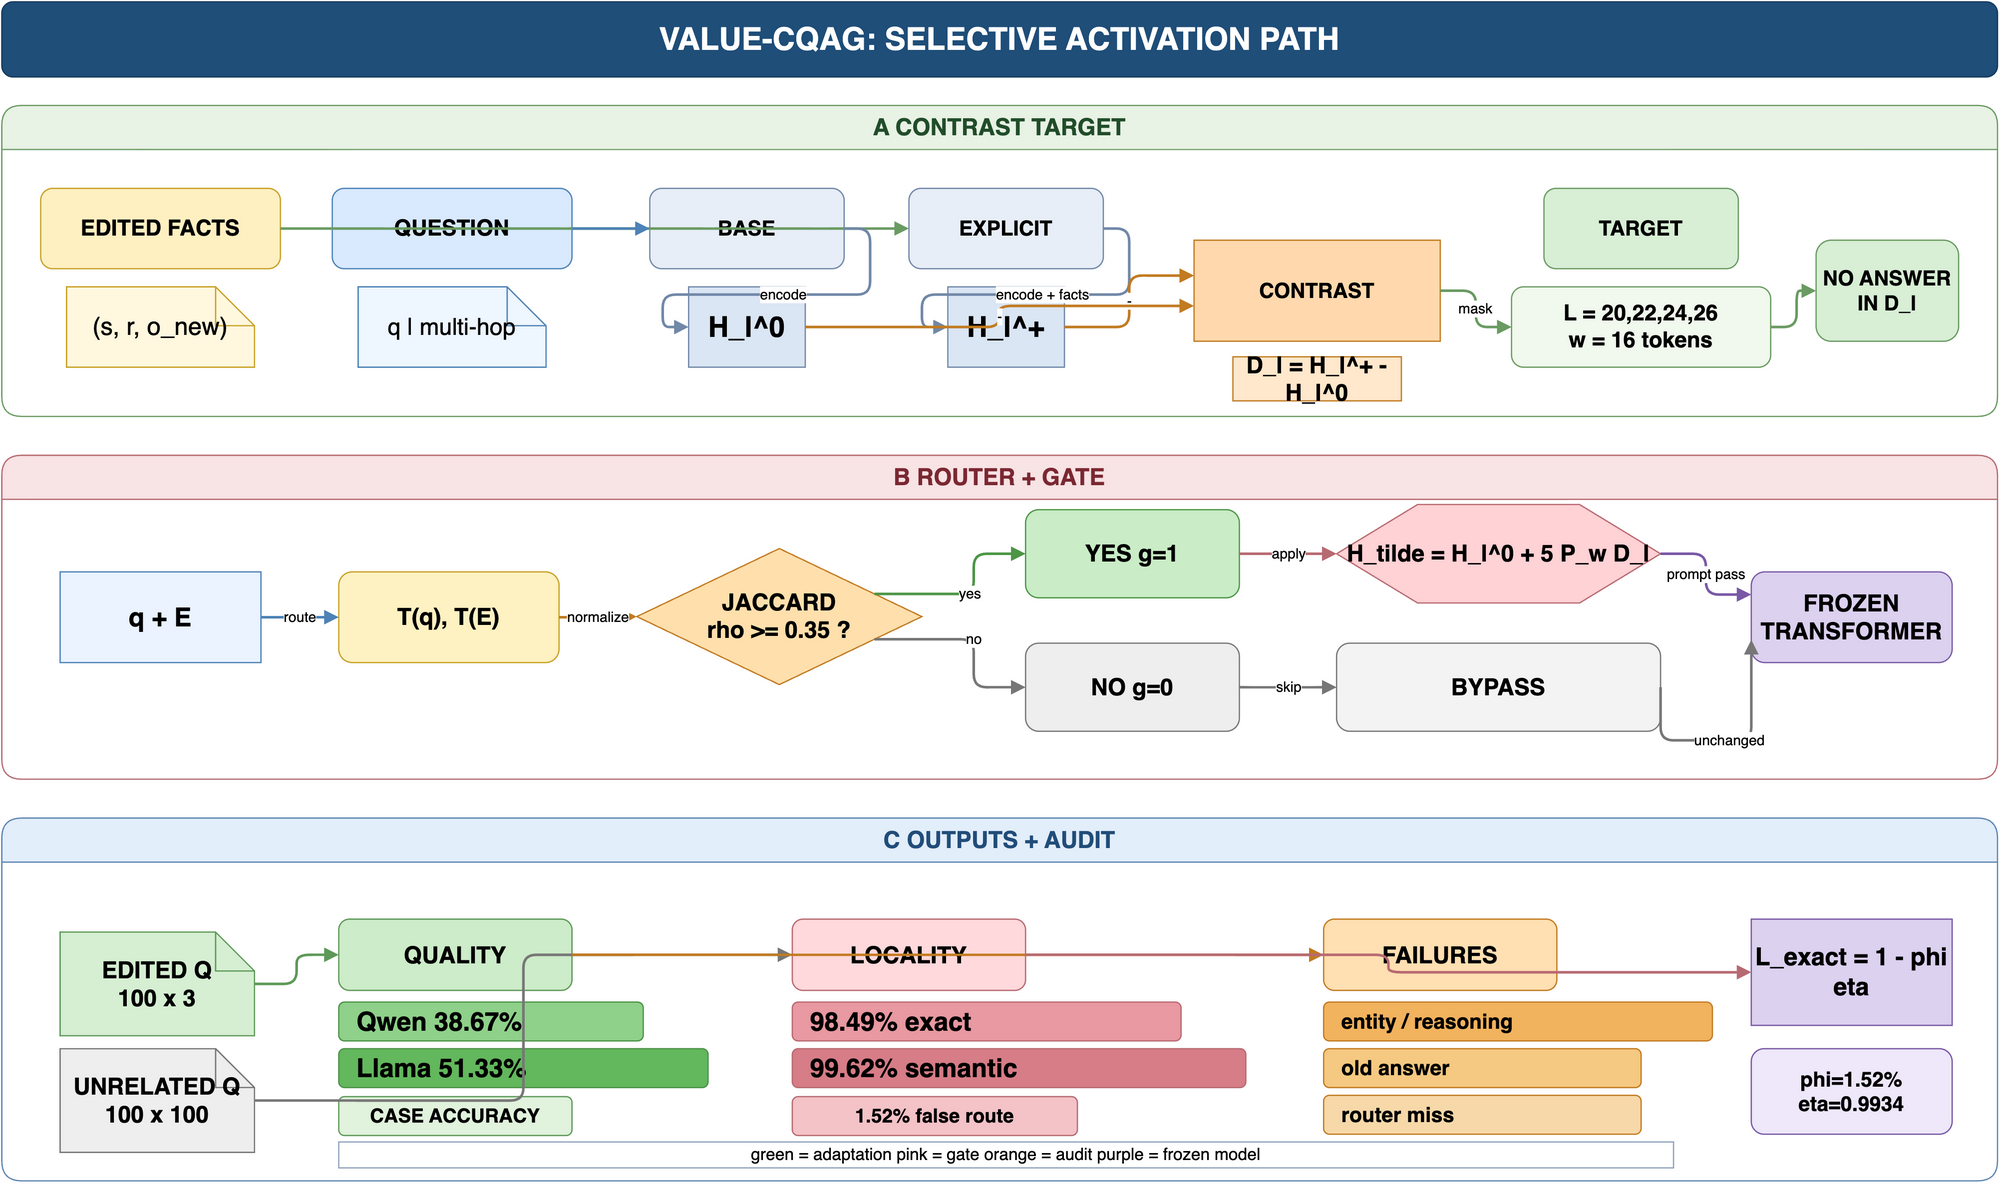
\includegraphics[width=\columnwidth]{cqag_pipeline.png}
    \caption{\method{} routes an edited context before prompt-only activation intervention. Edited and unrelated questions share the frozen model, while the evaluator measures both multi-hop answer quality and unchanged-output locality.}
    \label{fig:pipeline}
\end{figure}

\section{Experimental Protocol}
\subsection{Models and data}
We evaluate Qwen2.5-7B-Instruct and Llama-3.1-8B-Instruct. All principal comparisons use the same frozen 100-case MQuAKE-CF confirmation pool, containing 300 generated questions. The pool is kept separate from a reserved 60-case set that is not used in this study. For each edited case, five deterministic unrelated questions are used for the parameter-editing locality evaluation.

\subsection{Baselines and metrics}
We compare four adaptation modes: (i) the unmodified base model, (ii) explicit facts placed in the prompt, (iii) a transparent retrieval-plus-ICL control inspired by IKE \cite{zheng2023ike}, and (iv) EasyEdit \memit{} \cite{meng2023memit}. The retrieval corpus contains 500 non-overlapping development cases and uses MiniLM semantic retrieval with eight demonstrations. This is an IKE-style control, not a claim of an unmodified official IKE reproduction.

We report question-level generation accuracy, case-level generation accuracy (all questions in a case correct), new-answer preference, and exact-output locality. The routed locality audit contains 100 edited cases crossed with 100 unrelated questions, yielding 10,000 pairs. Exact locality requires an unchanged output string; semantic locality uses the task's semantic equivalence check. For \memit{}, locality is measured on 500 fixed unrelated outputs and is not directly pooled with the 10,000-pair router audit.

\subsection{Reproducibility}
For \memit{}, second-moment statistics use the local `wikimedia/wikipedia` 20231101.en mirror, 100,000 samples, float32, and layers 4--8 of `mlp.down\_proj`. Due to the 24-GB RTX 3090 memory limit, models are loaded in fp16; the covariance linear system is solved in CPU double precision and only the resulting update is moved to the GPU. The scripts, hparams, frozen IDs, and raw JSON artifacts accompany this paper draft.

\section{Results}
\subsection{Cross-model comparison}
Table~\ref{tab:main} shows the primary confirmation results. \method{} improves over the base model on both architectures, but explicit facts and retrieval remain stronger on answer accuracy. This separation is useful: the contribution is controlled adaptation and locality, not a claim that a short intervention prompt outperforms a large retrieval context.

\begin{table}[t]
\centering
\caption{Question-level and case-level generation accuracy on the same frozen confirmation pool. Retrieval+ICL$^{\dagger}$ was run on Qwen only, using eight demonstrations from 500 development cases.}
\label{tab:main}
\small
\begin{tabular}{llcc}
\toprule
Model & Method & Question & Case \\
\midrule
Qwen2.5-7B & Base & 2.00\% & 0.0\% \\
& \method{} & 38.67\% & 18.0\% \\
& Explicit facts & 95.00\% & 90.0\% \\
 & Retrieval+ICL$^{\dagger}$ & 95.00\% & 93.0\% \\
Llama-3.1-8B & Base & 4.00\% & 0.0\% \\
& \method{} & 51.33\% & 32.0\% \\
& Explicit facts & 93.00\% & 87.0\% \\
\bottomrule
\end{tabular}
\end{table}

Relative to the base model, the paired question-level gain is +36.67 percentage points for Qwen (95\% CI [29.33, 44.33]) and +47.33 points for Llama (95\% CI [39.33, 55.33]). Retrieval-plus-ICL reaches 95.0\% question-level and 93.0\% case-level accuracy on Qwen, but its exact and semantic locality are only 25.0\% and 61.4\%, respectively.

\subsection{Locality and parameter editing}
The end-to-end routed audit on Qwen gives a 1.52\% false-positive rate, 98.49\% exact-output locality, and 99.62\% semantic locality. Conditional on a false route, exact locality falls to 0.66\%, showing that the router is the main safety boundary. The audit records 37 newly corrupted originally-correct outputs and only one newly fixed originally-incorrect output.

Table~\ref{tab:edit} compares the two \memit{} runs. The method has lower generation accuracy than \method{} and substantially lower locality on Llama. These results indicate that a weight edit can provide a persistent change, but persistence is not equivalent to selective behavior on unrelated questions.

\begin{table}[t]
\centering
\caption{EasyEdit \memit{} on the frozen 100-case pool. Locality uses 500 unrelated outputs.}
\label{tab:edit}
\scriptsize
\setlength{\tabcolsep}{3pt}
\begin{tabular}{lccccc}
\toprule
Model & Pref. & Q-gen. & Case & Exact loc. & Edit (s) \\
\midrule
Qwen2.5-7B & 16.0\% & 16.0\% & 8.0\% & 85.2\% & 52.41 \\
Llama-3.1-8B & 18.0\% & 14.33\% & 5.0\% & 73.4\% & 29.64 \\
\bottomrule
\end{tabular}
\end{table}

\subsection{Failure decomposition}
Among 300 Qwen questions, 116 are correct, 133 are other-entity or reasoning errors, 31 retain the old answer, 19 are router misses, and one is a refusal. Llama yields 154 correct, 96 other-entity or reasoning errors, 30 old-answer residuals, 19 router misses, and one refusal. The identical router-miss count across models separates coverage from the downstream generation bottleneck: after a successful route, multi-hop entity selection remains the dominant failure mode.

\section{Discussion and Limitations}
The experiments support three restrained conclusions. First, conditional activation intervention can improve multi-hop factual adaptation on two instruction-tuned models without changing their parameters. Second, routing produces high system-level locality, but the intervention itself is not local after a false route. Third, retrieval is a strong accuracy control and should be included in any comparison; \method{} is preferable when selective, lightweight, and reversible adaptation is more important than maximizing answer accuracy.

The study has limitations. The confirmation pool has 100 cases and is not a broad pretraining-scale benchmark. The router uses lexical overlap and can miss paraphrases. The five-question parameter-editing locality protocol and 10,000-pair routed audit measure related but different quantities. Finally, the MEMIT implementation uses a hardware compatibility path (fp16 loading and CPU double solve) on a 24-GB GPU. We therefore report the exact protocol and do not claim an unmodified official MEMIT run.

\section{Conclusion}
We presented a cross-model study of locality-aware activation intervention for multi-hop factual adaptation. The key result is not a new accuracy record: it is a measured separation between adaptation quality, routing coverage, and unintended change. This separation makes failure analysis actionable and gives future work a concrete target: improve semantic routing and multi-hop composition while preserving the high locality of the gated path.

\balance
\bibliographystyle{IEEEtran}
\bibliography{references}
\end{document}
